\documentclass[14pt]{extarticle}
\usepackage{graphicx} % Required for inserting images
\usepackage{parskip}
\usepackage{amsmath}
\usepackage{amsthm}
\usepackage{amssymb}
\usepackage{bbm}
\usepackage{mathtools}
\usepackage{cleveref}
\usepackage{booktabs}
\usepackage{titlesec}
\usepackage{float}
\usepackage{fancyhdr}
\usepackage{stmaryrd}
\usepackage{logicproof}
\setlength{\parskip}{1em}
\setlength{\headheight}{17.0pt}
\usepackage{tikz}
\usetikzlibrary{arrows.meta,positioning}

\pagestyle{fancy}
\fancyhf{}
\fancyhead[R]{\thepage}

\newcommand{\impl}{\xrightarrow{}}
\newcommand{\ifff}{\longleftrightarrow}
\newcommand{\N}{\mathbbm{N}}
\newcommand{\R}{\mathbbm{R}}
\newcommand{\Q}{\mathbbm{Q}}
\newcommand{\A}{\mathbbm{A}}
\newcommand{\B}{\mathbbm{B}}
\newcommand{\Z}{\mathbbm{Z}}
\newcommand{\Sset}{\mathbbm{S}}
\newcommand{\X}{\mathbbm{X}}
\newcommand{\Pset}{\mathbbm{P}}
\newcommand{\powerset}{\mathcal{P}}
\newcommand{\pordereq}{\preceq}
\newcommand{\porder}{\prec}
\newcommand{\xor}{\bigoplus}

\newtheorem{theorem}{Theorem}

\title{\vspace{-2.5cm}Discrete Structures}
\author{Daksh Maahor}
\date{September 2025}

\begin{document}

\maketitle

\tableofcontents
\newpage

\section{Introduction : Propositions}

\subsection{Propositions}
\noindent A proposition is a statement which is either true or false (but not both).

\noindent Ex :- "It is raining in Mumbai today!!!" is a proposition, most probably true :( \\
\noindent Ex :- $x+3 = 8$ is not a proposition, as it cannot be determined to be true or false without fixing a value for $x$.

\noindent Similarly, since we use variables $x, y, z, \dots$ for numbers, we will use $p, q, r, \dots$ for propositions.

\subsection{Combining Propositions}
The propositions can be combined using Boolean operators such as $\neg$, $\land$, $\lor$, $\impl$, $\ifff$, etc.
\begin{align*}
    p &: \text{It is raining} \\
    \neg p &: \text{It is not raining} \\
    q &: \text{I will go to class} \\
    p \land \neg q &: \text{It is raining and I will not go to class} \\
    \neg p \impl q &: \text{If it is not raining then I will go to class}
\end{align*}

\subsection{Truth Tables!}
A Truth Table is a table that lists all the possible combinations of inputs and their corresponding outputs. For example:

\begin{table}[ht]
\centering
\begin{minipage}{0.45\textwidth}
  \centering
  \begin{tabular}{|c|c|c|}
    \hline
    $p$ & $q$ & $p \land q$ \\
    \hline
    0 & 0 & 0 \\
    0 & 1 & 0 \\
    1 & 0 & 0 \\
    1 & 1 & 1 \\
    \hline
  \end{tabular}
  \caption{Truth table for $p \land q$}
  \label{tab:first}
\end{minipage}%
\hspace{0.05\textwidth} % space between tables
\begin{minipage}{0.45\textwidth}
  \centering
  \begin{tabular}{|c|c|c|}
    \hline
    $p$ & $q$ & $p \lor q$ \\
    \hline
    0 & 0 & 0 \\
    0 & 1 & 1 \\
    1 & 0 & 1 \\
    1 & 1 & 1 \\
    \hline
  \end{tabular}
  \caption{Truth table for $p \lor q$}
  \label{tab:second}
\end{minipage}
\end{table}

\begin{table}[ht]
    \centering
    \begin{tabular}{|c|c|c|}
        \hline
        $p$ & $q$ & $p \xor q$ \\
        \hline
        0 & 0 & 0 \\
        0 & 1 & 1 \\
        1 & 0 & 1 \\
        1 & 1 & 0 \\
        \hline
    \end{tabular}
    \caption{Truth table for $p \xor q$}
    \label{tab:third}
\end{table}

\subsubsection{Important logical equivalences}
Logical equivalence means that the truth tables of two statements are identical.
Some important logical equivalences are:

\begin{itemize}
    \item $p \impl q$ is equivalent to $\neg p \lor q$
    \item $p \ifff q$ is equivalent to $(p \impl q) \land (q \impl p)$
\end{itemize}

\subsubsection{Operator Precedence}

The Operator Precedence of the Logical Operators follows the given order:

\[\neg \text{ then } \land \text{ then } \lor \text{ then } \impl \text{ then } \ifff\]
\newpage
Eg: Construct the truth table for $(p \lor \neg q) \impl (p \land q)$

\begin{table}[ht]
    \centering
    \begin{tabular}{|c|c|c|c|c|c|}
        \hline
        $p$ & $q$ & $\neg q$ & $p \lor \neg q$ & $p \land q$ & $(p \lor \neg q) \impl (p \land q)$ \\
        \hline
        0 & 0 & 1 & 1 & 0 & 0 \\
        0 & 1 & 0 & 0 & 0 & 1 \\
        1 & 0 & 1 & 1 & 0 & 0 \\
        1 & 1 & 0 & 1 & 1 & 1 \\
        \hline
    \end{tabular}
    \caption{Truth table for $(p \lor \neg q) \impl (p \land q)$}
    \label{tab:fourth}
\end{table}

\subsection{Negation, Converse and Contrapositive}
Take the following propositions:
\begin{align*}
        p:& \ \text{It will rain today} \\
        q:& \ \text{The match will be canceled} \\
        p \impl q :& \ \text{If it will rain today then the match will be canceled} \\
\end{align*}
The negation of an implication is given as:
\[
    \neg (p \impl q) \equiv \neg (\neg p \lor q) \equiv p \land \neg q
\]
For the above statements:
\[
    \neg (p \impl q) : \ \text{It will rain today and the match will not be canceled}
\]

The converse of an implication is given as:
\[
    \text{Converse of } (p \impl q) \text{ is } (q \impl p)
\]
For the above statements:
\[
    q \impl p : \ \text{If the match will be canceled then it will rain today}
\]

The contrapositive of an implication is given as:
\[
    \text{Contrapositive of } (p \impl q) \text{ is } (\neg q \impl \neg p)
\]
For the above statements:
\[
    \neg q \impl \neg p : \text{If the match won't be canceled then it won't rain today.}
\]

$p \impl q \equiv \neg q \impl \neg p$, that is an implication is logically equivalent to its contrapositive.

\subsection{Quantifiers}

Quantifiers are additional statements that provide context-specific information, such as the domain of discourse. Some common quantifiers are the following.

\begin{itemize}
    \item $\forall n$ stands for all values of n in the given domain
    \item $\exists n$ stands for there exists a value of n in the given domain
    \item $\in$ is "the element of" symbol
\end{itemize}

The negation of $\forall$ is $\exists$ and vice versa.

Ex : The negation of $\forall x \; P(x)$ is $\exists x \; \neg P(x)$

Ex : The negation of $\forall x \; (x^2 \geq x)$ is $\exists x \; (x^2 < x)$

\newpage

\section{Theorems and Proofs}

A theorem is a proposition that can be proved or disproved. At the basic level, there are two basic methods of proving theorems, Induction and Contradiction.

\subsection{Examples of some proofs}

\begin{theorem}
$\text{For all x} \in \N\text{, } x \text{ is even} \ifff x + x^2 - x^3 \text{ is even.}$
\end{theorem}

\begin{proof}
The proof proceeds in two directions.

\begin{itemize}
    \item Forward direction : $\forall x \in \N \text{, } x \text{ is even} \impl x + x^2 - x^3 \text{ is even.} $

    Let $x \in \N$ and $x$ be even.
    
    So, $\exists k \in \N \text{, } x=2k$.

    Then, 
    $x + x^2 - x^3 = 2k + (2k)^2 - (2k)^3 = 2k + 4k^2 - 8k^3 = 2(k + 2k^2 - 4k^3) = 2m$

    where, $m = k + 2k^2 - 4k^3$, thus $m \in \Z$, ie, $2 \ | \ x + x^2 - x^3$.

    So, $x + x^2 - x^3$ is even.
    
    \item Reverse direction : $\forall x \in \N \text{, } x + x^2 - x^3 \text{ is even} \impl x \text{ is even.}$

    It is easier to prove the contrapositive,

    $\forall x \in \N \text{, } x \text{ is odd} \impl x + x^2 - x^3 \text{ is odd.} $

    Let $x \in \N$ and $x$ be odd.
    
    So, $\exists k \in \N \text{, } x=2k+1$.

    Then $x + x^2 - x^3 = (2k+1) + (2k+1)^2 - (2k+1)^3 = (2k+1) + (4k^2+4k+1) - (8k^3 + 12k^2 + 6k + 1) = (-8k^3-8k^2+1) = 2m+1$ where $m = -4k^3-4k^2$, thus $m \in \Z$, i.e. $x + x^2 - x^3$ is odd.

    So, $x + x^2 - x^3$ is odd.
\end{itemize}

Hence, Proved.
\end{proof}

\begin{theorem}
    There are infinitely many primes.
\end{theorem}

\begin{proof}
    Suppose that there are finitely many primes, say, $p_1 < p_2 < p_3 < \dots < p_n$. We call the set of those primes $\Sset$.

    Now, let $k = (p_1p_2p_3\dots p_n) +1$.

    Then, $k$ when divided by any $p_r$ returns a remainder of 1. So $k$ is not divisible by any of the $p_r$'s.

    Also, $k > 1$ and $k > p_n$, so $k$ must not be prime. So, by the fundamental theorem of arithmetic, $k$ can be written as a product of primes.

    Now take any prime $p$ in that product. Since $p$ divides $k$, therefore $p \neq p_i$ for any $i \in \{1, 2, \dots, n\}$.

    So $p$ is a prime that is not in $\Sset$. But this contradicts our assumption that $\Sset$ is the set of all primes. 
    
    This means that our assumption was wrong, and thus, there are infinitely many primes.
\end{proof}

\newpage

\begin{theorem}
    $\sqrt{2}$ is irrational.
\end{theorem}

\begin{proof}
    Let us assume, for the sake of contradiction, that $\sqrt{2}$ is rational.

    That is,

    \[ \sqrt{2} = \frac{p}{q} \] for some \[ p, q \in \N, q\neq 0 \]

    where $p$ and $q$ are co-prime.

    Then,

    \[ 2 = \frac{p^2}{q^2} \]
    \[p^2 = 2q^2\]

    Thus $p^2$ is divisible by 2. Since 2 is prime, this implies that $p$ is divisible by 2. So,

    \[\exists k \in \N, p = 2k\]

    \[(2k)^2 = 2q^2\]
    \[4k^2 = 2q^2\]
    \[q^2 = 2k^2\]

    Thus $q^2$ is divisible by 2. Since 2 is prime, this implies that $q$ is divisible by 2.

    Thus, both $p$ and $q$ are divisible by 2. This contradicts the statement that $p$ and $q$ are co-prime. So, our assumption that $\sqrt{2}$ is rational is false.

    So, $\sqrt{2}$ is irrational.
\end{proof}

\begin{theorem}
    There exist irrational numbers $x$ and $y$, such that $x^y$ is rational.
\end{theorem}

\begin{proof}
    We have already proved that $\sqrt{2}$ is irrational.

    Let $x = y = \sqrt{2}$, consider $z = x^y$.

    \begin{itemize}
        \item If $z$ is rational, then we have found a pair of irrational $(x, y)$ such that $x^y$ is rational.
        \item If $z$ is irrational, then let $x = z$ and $y = \sqrt2$. Then, $x^y = {({(\sqrt{2})}^{\sqrt{2}})}^{\sqrt{2}} = (\sqrt{2})^2 = 2$, which is rational, then we have found a pair of irrational $(x, y)$ such that $x^y$ is rational.
    \end{itemize}
\end{proof}

The above proof is a non-constructive proof. It establishes that a mathematical object exists without providing a method to construct or identify it. Such proof techniques are quite powerful.

\newpage

\begin{theorem}
    $21$ divides $4^{n+1} + 5^{2n-1}$ whenever $n \in \Z^+$.
\end{theorem}

\begin{proof}
    \begin{itemize}
        \item Base Case: For $n = 1$
        \[ 4^{n+1} + 5^{2n-1} = 4^2 + 5^1 = 16 + 5 = 21 = 21 \times 1 \]
        Thus, $21$ divides $4^{n+1} + 5^{2n-1}$ for $n = 1$
        \item Induction Hypothesis: Let for $n=k$, $k \geq 1$, we have
        \[ 21 \text{ divides } 4^{k+1} + 5^{2k-1} \]
        So,
        \[ 4^{k+1} + 5^{2k-1} = 21m \text{ for some } m \in \Z\]
        \item Induction Step: For $n = k+1$
        \[ 4^{n+1} + 5^{2n-1} = 4^{(k+1)+1} + 5^{2(k+1)-1} \]
        \[ 4^{k+2} + 5^{2k+1} = 4(4^{k+1}) + 25(5^{2k-1})\]
        \[ 4^{k+2} + 5^{2k+1} = 4(21m - 5^{2k-1}) + 25(5^{2k-1})\]
        \[ 4^{k+2} + 5^{2k+1} = 4(21m) + 21(5^{2k-1})\]
        \[ 4^{k+2} + 5^{2k+1} = 21(4m + 5^{2k-1}) = 21p\]
        for \[p = 4m + 5^{2k-1}\]
    \end{itemize}

    Thus, by induction, we have $21$ divides $4^{n+1} + 5^{2n-1} \ \forall n \in \Z^+$
\end{proof}

The above proof technique is another powerful tool known as mathematical induction.
\newpage

\subsection{Mathematical Induction as an Axiom}

We can define the induction axiom as follows.

Let $P(n)$ be a property of non-negative integers. If
\begin{itemize}
    \item $P(i)$ is true (Base case)
    \item $\forall k\geq i$, $P(k) \impl P(k+1)$
\end{itemize}
Then, $P(n)$ holds $\forall n\in \Z^+, n\geq i$

Induction axiom can then be used to prove an important theorem in computer science known as the Well Ordering Principle.

\subsection{The Well Ordering Principle}

Every non-empty set of non-negative integers has a smallest element.

\begin{proof} \
    \begin{itemize}
        \item Base Case: For a set of $1$ non-negative integer, the integer itself is obviously the smallest element.

        \item Induction Hypothesis: For any set of $k$ non-negative integers, let there exist a smallest element.

        \item Induction Step: Consider any set of $k+1$ non-negative integers, say $S_0$. Let $n_0 \in S_0$. Now consider the set $S_1 = S_0-\{n_0\}$. $S_1$ is a set of $k$ non-negative integers, thus $S_1$ has a smallest element, say $n_1$.

        Now, if $n_1 < n_0$, then $n_1$ will be the smallest element of the set $S_0$. Else $n_0$ will be the smallest element of $S_0$. In either case, $S_0$ will have a smallest element.
    \end{itemize}

    Thus, $\forall n \in \Z^+,$ any finite set of $n$ non-negative integers will have a smallest element.

    For an infinite set of non negative integers $\X$, take for any $n$, $\X_n = \X \cap \{0, \dots, n\}$. Now since $\X$ is not $\phi$ and $\bigcup_{i=0}^\infty \X_i = \X$, there exists $n \in \N$ such that $\X_n \neq \phi$.

    Then by above proof, $\exists x \in \X_n, \forall u \in \X_n, x \leq u$. Also if $u \in \X - \X_n$, we have $u \notin \{0, \dots, n\}$ and thus, $x \leq n < u$ so $x \leq u \ \forall \ u \in \X$
\end{proof}

\subsection{Induction as a theorem : WOP implies Induction}

\begin{theorem}
    Let $P(n)$ be a property of non-negative integers. If
    \begin{itemize}
        \item $P(i)$ is true (Base case)
        \item $\forall k\geq i$, $P(k) \impl P(k+1)$
    \end{itemize}
    Then, $P(n)$ holds $\forall n\in \Z^+, n\geq i$
\end{theorem}

\begin{proof}
    We will use contradiction. Let us assume induction is not true. This means that,

    \begin{itemize}
        \item $P(i)$ is true (Base case)
        \item $\forall k\geq i$, $P(k) \impl P(k+1)$
    \end{itemize}

    But, $\exists n\in \Z^+, n\geq i,$ such that $P(n)$ is not true.

    Then consider $\Sset = \{ i\in\N | P(i) \text{ is not true}  \}$

    Since $\Sset$ is non-empty, by WOP it must have a smallest element. Let that element be $n_0$. So, $P(n_0)$ is not true. This implies that $P(i)$ is true $\forall i<n_0$. Thus $P(n_0-1)$ is true. Using our induction step, $P(n_0-1) \impl P(n_0)$, so $P(n_0)$ is true. This is a contradiction, and thus our assumption must be wrong.

    Thus, $\forall n\in \Z^+, n\geq i, P(n)$ is true.
\end{proof}

\begin{theorem}
    Any integer $> 1$ can be written as a product of prime numbers.
\end{theorem}

\begin{proof}
    Proof by Contradiction.

    Let us assume there exist \\ 
    $\Sset = \{ n\in \Z^+, n > 1 \ | \ n \text{ cannot be written as a product of primes} \}$

    Since $\Sset$ is non empty, there exists a smallest element in $\Sset$. Call it $n_0$.

    First $n_0$ can't be prime, as then it can be written as a product of primes as $n_0 = n_0$.

    So, $n_0$ can be written as

    $n_0 = a\times b$, where $1 < a, b < n$

    Since $a$ and $b$ are smaller than $n$, they can be written as a product of one or more primes.

    $a = p_1p_2p_3\dots p_k$ and $b = q_1q_2q_3\dots q_m$ for $k,m \geq 1$

    But then $n_0 = p_1p_2p_3\dots p_k.q_1q_2q_3\dots q_m$ which is a contradiction.

    Thus, any integer $> 1$ can be written as a product of prime numbers.
\end{proof}

\begin{theorem}
    Any integer $> 1$ can be written as a "unique" product of one or more primes.
\end{theorem}

\begin{proof}
    Let us assume that there exists an integer $ > 1$ that cannot be written as a "unique" product of one or more primes.

    Let us call the set of all such integers $\Sset$.
    Clearly, $\Sset \neq \phi$

    By WOP, there exists a smallest element in $\Sset$, say $s$.

    Then, $s = p_1\dots\dots p_n = q_1\dots\dots q_m$, 
    
    where each $p_i \neq q_j \ \forall i \in \{1, 2, \dots, n\} \text{ and } j \in \{1, 2, \dots, m\}$

    Without loss of generality, assume $p_1 < q_1$.
    Then, $s = p_1 \times P = q_1 \times Q$ for some $P > Q$.

    Then, $s - p_1Q = p_1 (P-Q) = (q_1 - p_1)Q < s$, which implies that $(q_1 - p_1) < s$ and $Q < s$.

    So $(q_1 - p_1)$ and $Q$ must have a unique prime factorization, and thus $p_1$ must occur in it.

    If $p_1$ occurs in the factorization of $Q$, then $p_1 = q_j$ violates our hypothesis.

    If $p_1$ occurs in the factorization of $q_1-p_1$, then $p_1$ must divide $q_1$ which contradicts the fact that both $p_1$ and $q_1$ are prime.

    Hence, we have a contradiction, which means that our original claim was false.
    Thus, any integer $> 1$ can be written as a unique product of one or more primes.
\end{proof}

\begin{theorem}
    For any $m, n \in \N, \ m\neq 0, , $ there exists a quotient $q$ and remainder $r$ $(q, r \in \N)$, such that

    \[ n = q\times m+r, \ \ 0 \leq r < m \]
\end{theorem}

\begin{proof}
    Fix any $m > 0$, we use strong induction on $n$.

    \begin{itemize}
        \item Base case : for $n = \{ 0, \dots, m-1 \}$
we have $n = 0 \times m + n$.

        Thus Base case follows.

        \item Induction Step : We will prove for all $k \geq m$

        Hypothesis : Let $\forall n \in \N, \ n \leq k, \ \exists q, r \in \N$ such that\\ $n = q \times m + r, \ 0 \leq r < m$

        Then consider $0 \leq k - m + 1 \leq k$, thus we can use the induction hypothesis on $k -m + 1$.

        $k - m + 1 = q' \times m + r', \ 0 \leq r' < m$

        Now select $q^* = q' + 1$ and $r^* = r'$, then

        $k + 1 = q^* \times m + r^*, \ 0 \leq r^* < m$
    \end{itemize}

    Thus, by induction, for any $m, n \in \N, \ m\neq 0, , $ there exists a quotient $q$ and remainder $r$ $(q, r \in \N)$, such that
    \[ n = q\times m+r, \ \ 0 \leq r < m \]
\end{proof}

\section{Basic Structures : Sets and Functions}

\subsection{Sets}

A set is an unordered collection of objects. The objects of a set are called its elements.

Formally, let $P$ be a property. Then, any collection of objects that satisfy $P$ is a set, i.e., $\Sset = \{ x \ | \ P(x) \}$

\subsection{Some properties of sets}

\begin{itemize}
    \item $\A \subseteq \B \ifff \forall x \in \A, (x \in \B)$
    \item $\A \times \B = \{ (a, b) \ | \ a \in \A \land b \in \B \}$
    \item $\A \cup \B = \{ x \ | \ x \in \A \lor x \in \B \}$
    \item $\A \cap \B = \{ x \ | \ x \in \A \land x \in \B \}$
    \item Empty set is denoted by $\phi$
    \item Power set of $\A = \powerset(\A) = \{X \ | \ X \subseteq \A\}$
    \item If $U$ is the universal set, then $\A^C = U - \A = \{ x \ | \ x \in U \land x \notin \A \}$
\end{itemize}

\newpage

\subsection{Functions}

Let $\A$ and $\B$ be two sets. A function $f$ from $\A$ to $\B$ is an assignment of exactly one element of $\B$ to each element of $\A$.

$f : \A \impl \B$ is a subset $R$ of $\A \times \B$ such that

\begin{enumerate}
    \item $\forall a \in \A, \exists b \in \B$ such that $(a, b) \in R$
    \item If $(a, b) \in R$ and $(a, c) \in R$ then $b = c$
\end{enumerate}

If $f : \A \impl \B$ is a bijective function, then we can define its inverse $f^{-1} : \B \impl \A$, defined as $f^{-1}(b) = a \ifff f(a) = b$

If $f$ is a bijection, then $f^{-1}(f(x)) = f(f^{-1}(x)) = x$, i.e. $fof^{-1} (x) = f^{-1}of(x) = x$

\subsubsection{Functions on finite sets}

If $\A$ and $\B$ are two finite sets such that $f : \A \impl \B$ is a function from $\A$ to $\B$ then,

\begin{itemize}
    \item $f$ is injective $\impl$ $|\A| \leq |\B|$
    \item $f$ is surjective $\impl$ $|\A| \geq |\B|$
    \item $f$ is bijective $\impl$ $|\A| = |\B|$
\end{itemize}

\newpage

\subsubsection{Some important theorems : True for both finite and infinite sets}

\begin{itemize}
    \item $(\exists\textbf{ bij} \text{ from } \A \impl \B \land \exists\textbf{ bij} \text{ from } \B \impl C) \impl (\exists\textbf{ bij} \text{ from } \A \impl C)$

    \item $(\exists\textbf{ bij} \text{ from } \A \impl \B) \impl (\exists\textbf{ bij} \text{ from } \B \impl \A)$

\end{itemize}

\begin{theorem} [Schroder-Bernstein Theorem]
        \[(\exists \textbf{inj} \text{ from } \A \impl \B \land \exists \textbf{inj} \text{ from } \B \impl \A) \impl (\exists \textbf{bij} \text{ from } \A \impl \B)\]
        \[(\exists \textbf{surj} \text{ from } \A \impl \B \land \exists \textbf{surj} \text{ from } \B \impl \A) \impl (\exists \textbf{bij} \text{ from } \A \impl \B)\]
\end{theorem}

\subsection{Infinite Sets}

\subsubsection{Definition of Infinite Set}

\begin{theorem}
    Let $\A$ be a set, and $b \notin \A$. $\A$ is infinite $\ifff$ $\exists \textbf{bij }$ from $\A \impl \A \ \cup \ \{b\} $ 
\end{theorem}

\begin{proof}
    If $\A$ is infinite, then $\A \neq \phi$, so let $a_0 \in \A$. Define $f(a_0) = b$.

    Now $\A - \{a_0\}$ is infinite, so $\A - \{a_0\} \neq \phi$, so let $a_1 \in \A - \{a_0\}$. Define $f(a_1) = a_0$.

    $\forall i \in \N$, $i \geq 1, \ \A - \{a_0, \dots, a_{i-1}\}$ is infinite and hence non-empty. Then, define $f(a_i) = a_{i-1}$.

    Collecting all such $a_i$'s, we get $\A' = \{a_i \in \A \ | \ i \in \N\}$, $\A' \subseteq \A$.

    Now, if $\forall a \in \A, a \notin \A'$, we define $f(a) = a$, then $f$ will become a bijection.
\end{proof}

\subsubsection{Important Takeaways}

\begin{itemize}
    \item Even if $\A, \B$ are infinite, $\A \subsetneq \B$, there can be a bijection from $\A \impl \B$. That is, $\A$ and $\B$ will have the same "cardinality".

    \item From any set $\A$, there is a surjection from $\A \impl \N$ (Most Important).

    \item Finite unions of countable sets are countable.

    \item To show that an infinite set $\Sset$ is countable, it is enough to show that:

    \begin{itemize}
        \item either $\exists \textbf{inj }$ from $\Sset \impl \N$
        \item or $\exists \textbf{surj }$ from $\N \impl \Sset$ 
    \end{itemize}
\end{itemize}

\subsection{Some Important Bijections on Infinite Sets}

\subsubsection{Bijection from $\Z \impl \N$}

\[
    f(x) = \begin{dcases}
        -2x & x \leq 0 \\
        2x-1 & x > 0
    \end{dcases}
\]

\subsubsection{Bijection from $\N \times \N \impl \N$}

\[
    f(a, b) = \frac{(a+b)(a+b+1)}{2} + b
\]

\subsubsection{Bijection from $\N \impl \N \times \N$}

\[
    f(x) = (a, b)
\]
where
\[
    x = 2^a (2b+1) - 1
\]

\subsubsection{Bijection from $\N \times \N \times \N \impl \N$}

\[
    f(a, b, c) =  \frac{\left(\frac{(a+b)(a+b+1)}{2} + b + c\right)\left(\frac{(a+b)(a+b+1)}{2} + b + c + 1\right)}{2} + c
\]

\subsubsection{Bijection from $\N \impl \N \times \N \times \N$}

\[
    f(x) = (a, b, c)
\]
where
\[
    x = 2^{(2^{a}(2b+1) - 1)}(2c+1) - 1
\]

\subsubsection{Proving the inexistence of a bijection}

\begin{theorem}
    There does not exist any bijection from $\R \impl \N$
\end{theorem}

\begin{proof}
    For the sake of contradiction, let us say that there exists a bijection, namely $f : \R \impl \N$. This means that we can enumerate all the real numbers in a table side by side of natural numbers. ie,
    \[
        \forall y \in \R \ \exists x \in \N, f(x) = y
    \]
    Let $a_i$ denote the digit at $10^{-(i+1)}$th place in $f(i)$, $i \in \N$. Define $b_i$ as
    \[
        b_i = \begin{dcases}
            a_i + 1 & a_i < 9 \\
            0 & a_i = 9
        \end{dcases}
    \]
    and then define a real number $p$ as
    \[
        p = \sum_{i = 0}^{\infty} b_i \times 10^{-(i+1)}
    \]
    Then, $p - f(i) \neq 0$, ie, $p \neq f(i) \ \forall i \in \N$

    But this contradicts our original claim that $f$ is a bijection. Thus, our assumption must be wrong, and so, there does not exist any bijection from $\R \impl \N$
\end{proof}

Similarly we can prove the inexistence of bijection from $\powerset(\N) \impl \N$.

\subsubsection{Proving the existence of a bijection}

\begin{theorem}
    There exists a bijection from $\R \impl \powerset{(\N)}$.
\end{theorem}

\begin{proof}
    First we show there exists a bijection from $\R \impl (0, \ 1)$.

    Consider the function:

    \[
        f(x) = \frac{1}{2} + \frac{1}{\pi}\tan^{-1}{(x)}
    \]

    This function is continuous, strictly increasing and maps $\R$ to $(0, \ 1)$. Thus, this function is a bijection.

    Next we construct a bijection from $(0, \ 1) \impl (0, \ 1) \cup \N$ as:

    \[
        g(x) = \begin{dcases}
            n-1 & x = \frac{1}{n+1}; \ n \in \N, \ n \geq 1 \\
            \frac{(k-1)n+1}{kn+1} & x = \frac{kn+1}{(k+1)n+1}; \ k,\ n \in \N, \ n \geq 1, \ k \geq 1 \\
            x & \text{otherwise}
        \end{dcases}
    \]

    This function basically creates partitions of rationals into sets of all such $\frac{p}{q}$ whose $q-p=c$ is constant. Then it maps the smallest element of each partition to $c-1$, and then progressively maps the next element to the current element. For irrationals, it maps the number to itself.

    Proving that the function is well defined and indeed a bijection is left as an exercise to the reader :)

    Next we create a bijection from $(0, \ 1) \cup \N \impl \powerset(\N)$

    Define a function $h : (0, \ 1) \cup \N \impl \powerset(\N)$ as:

    \begin{itemize}
        \item $h(0) = \phi$, $h(1) = \N$
        \item For $n \in \N, \ n>1$, construct a set $\Sset_n$ as:
        \[
            \Sset_n = \{k \ | \ (k+1)^{th} \text{ bit from the right of n in base 2 is 1.}\}
        \]
        Eg: For 37, base 2 representation is $(100101)_2$, and thus the set $S_{37} = \{0, \ 2, \ 5\}$
        \item For $x \in (0, \ 1)$, we use the non terminating binary representation of $x$. Every number in $(0, \ 1)$ can be represented in binary as $0.b_0b_1b_2\dots$ where $b_i \in \{0,\ 1\}$.
        We then construct the set as:
        \[
            \Sset_x = \{k \ | \ b_k = 1\}
        \]
        Note : If the binary representation has only finite significant digits, we will enforce it to have infinite. Eg: $(0.65625)_{10} = 0.10101 = 0.1010011111111\dots$
        Thus, $S_{0.65625} = \{0, 2, 5, 6, 7, \dots\}$
    \end{itemize}

    Finally,
    \[
        h(x) = \begin{dcases}
            \phi & x = 0 \\
            \N & x = 1 \\
            \Sset_n & x = n, \ n \in \N, n \geq 2 \\
            \Sset_x & x \in (0, \ 1)
        \end{dcases}
    \]
    Then the required bijection from $\R \impl \powerset{(\N)}$ will be given as $\mathcal{H}(x) = h(g(f(x))) : \R \impl \powerset(\N)$
\end{proof}

\subsubsection{Cartesian product of countable sets}

\begin{theorem}
    Cartesian product of countable sets is countable.
\end{theorem}

\begin{proof}
    Let $\A$ and $\B$ be countably infinite. Then define a bijection $f \ : \ \A \times \B \impl \N$ as

    \[
        f(a_i, \ b_j) = (\sum_{k = 1}^{i+j} k) + j
    \]
\end{proof}

\subsubsection{Are Rationals countable??}

\begin{theorem}
    There exists a bijection from $\Q \impl \N$
\end{theorem}

\begin{proof}
    First, we will show that there exists an injection from \\ $\Q \impl \N$.

    Let the rational number be given as $s \times \frac{p}{q}$ where $p$, $q$ $\in \N$ and are co-prime, $q \neq 0$ and $s = -1$ or $1$ depending on the sign of the rational number.

    Consider the mapping,

    \[
        f(s \times \frac{p}{q}) = 2^p3^q5^{s+1}
    \]

    The fundamental theorem of arithmetic guarantees that the above mapping is injective. So, there exists an injection from $\Q \impl \N$.

    Also, since $Q$ is infinite, we also know that there exists an injection from $\N \impl \Q$. Thus by Schroder-Bernstein Theorem, there exists a bijection from $\Q \impl \N$.

    Thus, rationals are countable.
\end{proof}

\subsection{Cantor's Theorem and Cantor's Continuum Hypothesis}

\begin{theorem}[Cantor's Theorem]
    There exists no bijection from $\N \impl \powerset(\N)$. Since there exists a surjection from $\powerset(\N) \impl \N$, the cardinality of $\powerset{(\N)}$ is strictly greater than that of $\N$.
\end{theorem}

Cantor's continuum hypothesis states that there exists no set whose cardinality is strictly between $\N$ and $\powerset(\N)$.


\subsection{Relations}

A Relation $R$ from $\A \impl \B$ is a subset of $\A \times \B$. If $(a, \ b) \in R$, then we can write it as $a \ R \ b$. All functions are relations but not all relations are functions.

\subsubsection{Partitions of a set}

A partition of a set $\Sset$ is a set $\Pset \subset \powerset{(\Sset)}$ such that:

\begin{itemize}
    \item $\Sset' \in \Pset \impl \Sset' \neq \phi$
    \item $\bigcup\limits_{\Sset' \in \Pset} \Sset' = \Sset$, ie, the union of the elements of a partition covers the entire set.
    \item If $\Sset_1, \ \Sset_2 \in \Pset$, then $\Sset_1 \cap \Sset_2 = \phi$, ie, the sets are disjoint.
\end{itemize}

If we define a partition on a set and then define a relation such that all elements in a partition are related to each other, we get a special type of relation.

\subsubsection{Relation generated by partitions}

Relations generated by partitions follow some special properties :

\begin{itemize}
    \item Reflexivity : $\forall a \in \A , \ (a, \ a) \in R$
    \item Symmetry : $\forall a, \ b \in \A, \ (a, \ b) \in R \impl (b, \ a) \in R $
    \item Transitivity : $\forall a, \ b, \ c \in \A, \ (a, \ b) \in R \ \land \ (b, \ c) \in R \impl (a, \ c) \in R$
\end{itemize}

A relation satisfying the above conditions is called an equivalence relation. Thus, from a partition we get an equivalence relation.

\subsubsection{Equivalence Classes}

Let $R$ be an equivalence relation on set $\Sset$, and let $a \in \Sset$. The equivalence class of $a$, denoted as $[a]$ is defined as,

\[
    [a] = \{b \in \Sset \ | \ (a, \ b) \in R\}
\]

\begin{theorem}
    \[
        aRb \ifff [a] = [b] \ifff [a] \cap [b] \neq \phi
    \]
\end{theorem}

\begin{theorem}
    If $R$ is an equivalence relation on $\Sset$, then the equivalence classes of $R$ form a partition of $\Sset$. In contrast, given a partition $P$ of a set $\Sset$, there exists an equivalence relation $R$ whose equivalence classes are exactly the sets of $P$.
\end{theorem}

The proof of above theorem is quite simple and hence, left as an exercise to the reader.

\subsubsection{Defining new Objects through equivalence relations}

\begin{itemize}
    \item Consider $R = \{((a, \ b), \ (c, \ d) \ | \ (a, \ b), \ (c, \ d) \in \Z \times \Z/\{0\},  \ (ad = bc) \}$

    Then the equivalence classes of $R$ define rational numbers. Eg: $(2, \ 4) \in [(1, \ 2)]$ is equivalent to saying $\frac{2}{4} = \frac{1}{2}$

    Similarly, equivalence classes of \\ $R = \{((a, \ b), \ (c, \ d) \ | \ (a, \ b), \ (c, \ d) \in \N \times \N,  \ (a+d = b+c) \}$ define integers.

    \item Consider the relation\\ $R([0, 1]) = \{ aRb \ | \ a, b \in [0, 1], a = b \text{ or } (a, b) = (0, 1) \text{ or } (1, 0)\}$

    If we imagine the interval $[0, 1]$ as a thread of length 1, then the above relation describes a loop where we have glued the ends of the thread.

    \item Consider the relation\\ $R([0, 1] \times [0, 1]) = \{ (a, b)R(c, d) \ | \ (a, b) = (c, d) \text{ or } b = d, c = 0, a = 1 \text{ or } b = d, a = 0, c = 1 \}$

    Imagining $[0, 1] \times [0, 1]$ as a square of side 1, the above relation describes joining the two vertical sides of the square together to form a cylinder.

    \item Similarly we can describe a torus through relations. Give it a try!
    

    \textbf{Spoiler:}

    Consider the relation\\ $R([0, 1] \times [0, 1]) = \{ (a, b)R(c, d) \ | \ (a, b) = (c, d) \text{ or } b = d, c = 0, a = 1 \text{ or } b = d, a = 0, c = 1 \text{ or } a = c, b = 0, d = 1 \text{ or } a = c, d = 0, b = 1 \text{ or } a, b, c, d \in \{0, 1\} \}$
\end{itemize}

\newpage

\section{Basic Structures : Posets}

\subsection{Anti-Symmetry}

Consider the relation $R = \{ (a, b) \ | \ a, b \in \Z, a \leq b \}$. This relation is reflexive and transitive but not symmetric. In fact, it is "Anti-Symmetric".

A relation $R$ on a set $\Sset$ is called anti-symmetric if $\forall \ a, b \in \Sset$, $(aRb \ \land \ bRa) \impl a = b $.

Examples of anti-symmetric relations are:

\begin{itemize}
    \item $R(\Z) = \{(a, b) \ | \ a, b \in \Z, \ a \leq b\}$
    \item $R(\powerset(\Sset)) = \{(\A, \B) \ | \ \A, \B \in \powerset(\Sset), \ \A \subseteq \B\}$
\end{itemize}

\subsection{Partial Orders}

A Partial Order is a relation which is reflexive, transitive and anti-symmetric. Partial orders are denoted by $a \pordereq b$ instead of $aRb$. 

There can be a case where some elements in a partial order may not be comparable by the operator defined by the order. That is why it is called a partial order.

A Total Order is then a Partial Order $\pordereq$ on a set $\Sset$ in which every pair of elements is comparable.

In the above two examples, the first one is a total order while the second one is not (can you see why?).

\newpage

\subsection{Partially Ordered Sets : Posets}

A set $\Sset$ together with a partial order $\pordereq$ defined on it, is called a partially ordered set, or a poset, denoted as $(\Sset, \pordereq)$.

Examples of Posets : $(\Z, \ \leq)$, $(\Z^+, \ | \ )$, $(\powerset(\Sset), \ \subseteq)$ etc.

\subsubsection{Graphical Representation of a Poset}

Posets can be represented graphically as shown :

Graph of the Poset $(\powerset(\{1, 2, 3\}), \ \subseteq)$


\begin{center}
\begin{tikzpicture}[
  every node/.style={draw, rectangle, minimum width=1.4cm, inner sep=2pt, align=center},
  node distance=1.8cm and 2.4cm,
  >=Latex
]

% --- Nodes (each drawn once) ---
\node (0) {$\phi$};

\node (1)   [above left=of 0] {$\{1\}$};
\node (2)   [above=of 0]      {$\{2\}$};
\node (3)   [above right=of 0]{$\{3\}$};

\node (12)  [above left=of 2] {$\{1,2\}$};
\node (13)  [above=of 2]      {$\{1,3\}$};
\node (23)  [above right=of 2]{$\{2,3\}$};

\node (123) [above=of 13]     {$\{1,2,3\}$};

% --- Self loops ---
\foreach \n/\pos in {0/below,1/left,2/below,3/right,12/left,13/above,23/right,123/above}
  \draw[->] (\n) edge[loop \pos, looseness=10, min distance=8] (\n);

% --- All comparability edges ---

% from empty set to singletons
\draw[->] (0) to[out=100,in=-150] (1);
\draw[->] (0) to[out=90,in=-90]   (2);
\draw[->] (0) to[out=80,in=-30]   (3);

% from empty set to pairs
\draw[->] (0) to[out=70,in=-170]  (12);
\draw[->] (0) to[out=135,in=-130]  (13);
\draw[->] (0) to[out=110,in=-10]  (23);

% from empty set to top
\draw[->] (0) to[out=60,in=-60,looseness=1.5] (123);

% singletons to pairs
\draw[->] (1) to[out=70,in=-150] (12);
\draw[->] (1) to[out=60,in=-160] (13);

\draw[->] (2) to[out=100,in=-120] (12);
\draw[->] (2) to[out=80,in=-100]  (23);

\draw[->] (3) to[out=120,in=-40]  (23);
\draw[->] (3) to[out=100,in=-20]  (13);

% singletons to top
\draw[->] (1) to[out=70,in=-140]  (123);
\draw[->] (2) to[out=140,in=-120,looseness=1.3]   (123);
\draw[->] (3) to[out=110,in=-40]  (123);

% pairs to top
\draw[->] (12) to[out=80,in=-120] (123);
\draw[->] (13) to[out=90,in=-90]  (123);
\draw[->] (23) to[out=100,in=-60] (123);

\end{tikzpicture}
\end{center}

The above directed tree becomes a bit messy for bigger posets. Thus we draw what is called a "Hasse Diagram" to keep things neat.

\begin{center}
\begin{tikzpicture}[
  every node/.style={draw, rectangle, minimum width=1.2cm, align=center},
  node distance=1.8cm and 2cm
]

% Level 0
\node (0) {$\phi$};

% Level 1
\node (1)   [above left=of 0] {$\{1\}$};
\node (2)   [above=of 0]      {$\{2\}$};
\node (3)   [above right=of 0]{$\{3\}$};

% Level 2
\node (12)  [above left=of 2] {$\{1,2\}$};
\node (13)  [above=of 2]      {$\{1,3\}$};
\node (23)  [above right=of 2]{$\{2,3\}$};

% Level 3
\node (123) [above=of 13]     {$\{1,2,3\}$};

% Edges
\draw[->] (0) -- (1);
\draw[->] (0) -- (2);
\draw[->] (0) -- (3);

\draw[->] (1) -- (12);
\draw[->] (1) -- (13);
\draw[->] (2) -- (12);
\draw[->] (2) -- (23);
\draw[->] (3) -- (13);
\draw[->] (3) -- (23);

\draw[->] (12) -- (123);
\draw[->] (13) -- (123);
\draw[->] (23) -- (123);

\end{tikzpicture}
\end{center}

In a Hasse diagram, the edges showing reflexivity and transitivity are omitted. We show only those $x \pordereq y$ where there exists no $z$ such that $x \pordereq z \pordereq y$. The reflexive-transitive closure of the Hasse diagram gives back the original graph of the poset.

\subsection{Chains and Anti-Chains}

\subsubsection{Chains}

Let $(\Sset, \pordereq)$ be a poset. Then a subset $\A \subseteq \Sset$ is called a chain if
\[
    \forall a, \ b \in \A, \ a \pordereq b \ \lor \ b \pordereq a
\]
That is, all pair of elements must be related to each other through the partial order. In other words, \textbf{a chain is a totally ordered subset of some partial order.}

\subsubsection{Anti-Chains}

Let $(\Sset, \pordereq)$ be a poset. Then a subset $\A \subseteq \Sset$ is called an anti-chain if
\[
    \forall a, \ b \in \A, a\neq b,  \ \neg (a \pordereq b) \ \land \ \neg (b \pordereq a)
\]
That is, none of the elements in an anti-chain are related to each other through the partial order.

Example : In poset $(\{1, 2, 3\}, \ \subseteq)$, the set $\{ \ \phi, \{1\}, \{1, 2\}, \{1, 2, 3\} \ \}$ is a chain while the set $\{ \ \{1, 2\}, \{2, 3\}, \{1, 3\} \ \}$ is an antichain.

\subsection{Topological Sort}

A Topological Sort or Linearization of a poset $(\Sset, \pordereq)$ is a totally ordered set $(\Sset, \pordereq_t)$ with a total order $\pordereq_t$ defined on it such that $x \pordereq y \impl x \pordereq_t y$.

\subsubsection{Minimal Element}

An element $x$ in a poset is called a minimal element if there is no element $\nexists y \in \Sset, y \porder x$.

\begin{theorem}
    Every finite non-empty poset has a set of minimal elements.
\end{theorem}

\begin{proof}
    We will prove this theorem using induction.

    \begin{itemize}
        \item Base case : Consider a poset of 1 element, $(\Sset_1 = \{a_1\}, \pordereq)$

        Here $a_1$ is the minimal element $\nexists b \in \Sset_1, \ b \porder a_1$.

        Thus, the base case is satisfied.

        \item Induction hypothesis : Let any poset of k elements, \newline $(\Sset_k = \{a_1, \dots, a_k\}, \pordereq), \ k \geq 1$ have a set of minimal elements.

        \item Induction step : Consider any poset of k+1 elements,
        \newline
        $(\Sset_{k+1} = \{ a_1, \dots, a_k, a_{k+1} \}, \pordereq)$

        Now consider the poset obtained by removing the element $a_{k+1}$ from this poset, ie, $(\Sset'_{k+1} = \Sset_{k+1} -\{a_{k+1}\} = \{ a_1, \dots, a_k \}, \pordereq)$

        By our induction hypothesis, there exists a set of minimal elements in $\Sset'_{k+1}$, let that be $\X = \{l_1, \dots, l_n\}$, ie, $\forall b \in \Sset'_{k+1} \ \exists l_i \in \X, l_i \pordereq b$.

        Now, there are the following cases:

        \begin{enumerate}
            \item $\exists l_i \in \X, \ l_i \pordereq a_{k+1}$, in which case, that $l_i$ will still be a minimal element.
        
            \item Either $a_i$ and $a_{k+1}$ are incomparable in the poset $\Sset_{k+1}$. In that case $a_i$ would still be a minimal element as both $a_{k+1} \pordereq a_i$ and $a_i \pordereq a_{k+1}$ are false, and thus $\nexists b \in \Sset_{k+1}, b \porder a_i$.

            \item $a_i \pordereq a_{k+1}$ in which case $a_i$ would still be a minimal element as $\nexists b \in \Sset_{k+1}, b \porder a_i$.

            \item $a_{k+1} \pordereq a_i$ in which case $a_{k+1}$ would become a minimal element as, by transitivity, $a_{k+1} \pordereq a_i \ \impl \ \forall b \in \Sset_{k+1}, (a_i \pordereq b \impl \ a_{k+1} \pordereq b)$, and thus $\nexists b \in \Sset_{k+1}, \ b \porder a_{k+1}$.
        \end{enumerate}

        Thus, if a poset of size k has a minimal element, then a poset of size k+1 also has a minimal element.
    \end{itemize}

    Thus, by induction, we conclude that every finite non-empty poset has a minimal element.
\end{proof}

The above lemma can then be used to prove another important theorem.

\begin{theorem}
    Every finite non-empty poset has a topological sort.
\end{theorem}

\begin{proof}
    Let there be a finite non-empty poset $(\Sset, \pordereq)$ of n elements. We give an inductive algorithm to construct a topological sort:
    \begin{itemize}
        \item Start with the minimal element of $\Sset$, say $x_1$. This is a chain consistent with $\pordereq$.

        \item Suppose that we have already constructed a chain of $k$ elements $(1 \leq k < n)$ consistent with $\pordereq$, $x_1 \pordereq_t \dots \pordereq_t x_k$.

        \item Consider the poset $\Sset' = \Sset - \{a_1, \dots, a_k \}$. Let us say its minimal element is $x_{k+1}$.

        \item Then $x_1 \pordereq_t \dots \pordereq_t x_k \pordereq_t x_{k+1}$ is a chain of $k+1$ elements consistent with $\pordereq$. If not, then $\exists i \in \{1, \dots, k\}, \ x_{k+1} \pordereq x_i$, but $x_i \pordereq_t x_{k+1}$, but then it violates the minimality of $x_i$ at the $i^{th}$ step.

        \item Thus, after n steps we get a chain of n elements $x_1 \pordereq_t \dots \pordereq_t x_n$ consistent with our partial order $\pordereq$.
    \end{itemize}

    Using this algorithm, we can generate a topological sort of any finite non-empty poset, and hence there must exist a topological sort on every finite non-empty poset.
\end{proof}

\subsubsection{Parallel Task Scheduling}

For any non-empty and finite poset, there is a legal parallel schedule that runs in t steps, where t is the size of the longest chain.

This result is infact the consequence of the following theorem:

\begin{theorem}
    For a non-empty, finite poset $(\Sset, \pordereq)$ with size of longest chain $= t$, we can partition $\Sset$ into $t$ subsets $\Sset_1, \dots, \Sset_t$ such that $\forall i \in \{1, \dots, t\}$, $\forall a \in \Sset_i$, $b \porder a \impl b \in \Sset_1 \cup \dots \cup \Sset_{i-1}$
\end{theorem}

\begin{proof}
    Place each $a \in \Sset$ in $\Sset_i$ where $i$ is the length of the longest chain that ends at $a$.

    Now suppose $\exists i, a \in S_i, \ b \porder a$ but $b \notin \Sset_1 \cup \dots \cup \Sset_{i-1}$.

    By the definition of $\Sset_i$, $\exists$ a chain of size at least $i$ that ends at b.

    But then $b \porder a$ implies that we can extend that chain to another chain of size $i+1$ ending at a.

    But that contradicts the fact that $a \in \Sset_i$

    Thus $\forall a \in \Sset_i$, $b \porder a \impl b \in \Sset_1 \cup \dots \cup \Sset_{i-1}$
\end{proof}

Using this theorem, we can then schedule all tasks in $\Sset_i$ at time $i$ (since all previous tasks were done earlier!). So, each $\Sset_i$ is an anti-chain.

Since each $\Sset_i$ is an anti-chain, the above theorem was restated in a different way as Mirsky's Theorem.

\begin{theorem}[Mirsky's Theorem]
    If the largest chain in a poset $(\Sset, \pordereq)$ is of size $t$, then $\Sset$ can be partitioned into $t$ anti-chains.
\end{theorem}

And as a consequence of the above theorem comes the below corollary.

\begin{theorem}[Dilworth's Lemma]
    $\forall t > 0$ any poset with $n$ elements must have either a chain of size greater than $t$ or an anti chain with at least $\left \lceil \frac{n}{t} \right \rceil$ elements.
\end{theorem}

The proofs of the above theorems are trivial and hence left as an exercise to the reader :)

\subsection{Minimal and maximal elements}

Let $(\Sset, \pordereq)$ be a poset. 

An element $a$ of $\Sset$ is a minimal element of the poset if $\forall b \in \Sset, b \pordereq a \impl b = a$.

An element $a$ of $\Sset$ is a maximal element of the poset if $\forall b \in \Sset, a \pordereq b \impl a = b$.

An element $a$ of $\Sset$ is the least element of the poset if $\forall b \in \Sset, a \pordereq b.$

An element $a$ of $\Sset$ is the greatest element of the poset if $\forall b \in \Sset, b \pordereq a.$

\subsubsection{Upper Bounds and Lower Bounds}

Let $(\Sset, \pordereq)$ be a partially ordered set, and $\A \subseteq \Sset$.

An element $u \in \Sset$ is called an upper bound for $\A$ if $\forall a \in \A, a \pordereq u$.

An element $l \in \Sset$ is called a lower bound for $\A$ if $\forall a \in \A, l \pordereq a$.

An element $u \in \Sset$ is called a least upper bound for $\A$ if it is an upper bound and for all upper bounds $u'$, $u \pordereq u'$.

An element $l \in \Sset$ is called a greatest lower bound for $\A$ if it is a lower bound and for all lower bounds $l'$, $l' \pordereq l$.

\end{document}


